%% ============================================================================
%%  Cost-Aware Eviction for LLM Response Caching:
%%  A GDSF-Based Approach for GPTCache
%%
%%  Author : Nissim Brami  <nissimbrami@post.bgu.ac.il>
%%  Course : Caching in LLMs -- Ben-Gurion University of the Negev
%%  Repo   : https://github.com/nissimbrami/caching-course-project
%%
%%  Build:
%%      latexmk -pdf report.tex
%%  or  compile on Overleaf with pdfLaTeX (main = report.tex, bib = references.bib).
%% ============================================================================
\documentclass[sigconf, nonacm, review=false, screen=true]{acmart}

%% -- Metadata & packages -----------------------------------------------------
\usepackage{booktabs}
\usepackage{graphicx}
\usepackage{amsmath}
\usepackage{siunitx}
\usepackage{enumitem}
\usepackage{listings}
\usepackage{xcolor}
\usepackage{url}
\usepackage{hyperref}
\hypersetup{colorlinks=true, linkcolor=blue!60!black, citecolor=blue!60!black, urlcolor=blue!60!black}

\graphicspath{{figures/}}

%% -- Suppress conference footer (course project, not a real venue) -----------
\settopmatter{printacmref=false, printccs=false, printfolios=true}
\renewcommand\footnotetextcopyrightpermission[1]{}
\pagestyle{plain}

%% -- Code listing style ------------------------------------------------------
\definecolor{codegray}{gray}{0.95}
\lstdefinestyle{pystyle}{
    backgroundcolor=\color{codegray},
    basicstyle=\ttfamily\footnotesize,
    keywordstyle=\color{blue!60!black}\bfseries,
    commentstyle=\color{gray!70!black}\itshape,
    stringstyle=\color{orange!70!black},
    numbers=left, numberstyle=\tiny\color{gray}, numbersep=6pt,
    frame=single, framesep=4pt, rulecolor=\color{gray!30},
    breaklines=true, showstringspaces=false, tabsize=4,
    language=Python,
}
\lstset{style=pystyle}

%% -- Title & author ----------------------------------------------------------
\title{Cost-Aware Eviction for LLM Response Caching: \\
       A GDSF-Based Approach for GPTCache}

\author{Nissim Brami}
\affiliation{%
  \institution{Ben-Gurion University of the Negev}
  \department{Department of Computer Science}
  \city{Beer-Sheva}
  \country{Israel}
}
\email{nissimbrami@post.bgu.ac.il}

%% -- CCS / keywords ----------------------------------------------------------
\keywords{semantic caching, LLM inference, eviction policy,
          Greedy-Dual-Size-Frequency, GPTCache, cost-aware caching}

\begin{document}

\begin{abstract}
LLM API calls are among the most expensive operations in modern AI stacks:
per-query costs of a few cents accumulate quickly at scale. Semantic caching
systems such as GPTCache reduce those costs by reusing prior responses, but
their default eviction policies (LRU and FIFO) treat every cached entry as
equally valuable~---~which they are not. A cached response for an expensive
GPT-4 completion is worth far more than a cached response for a short
GPT-3.5 answer. We implement a cost-aware eviction policy based on the
Greedy-Dual-Size-Frequency (GDSF) algorithm~\cite{cherkasova1998gdsf,
cao1997costaware} from the classical web-proxy caching literature, and
evaluate it as a plugin for GPTCache~\cite{gptcache}. Each entry receives
priority $\text{Priority}(i) = L + \tfrac{\text{freq}(i)^\alpha \cdot
\text{cost}(i)^\beta}{\text{size}(i)}$, where the clock $L$ advances to the
priority of the last evicted item, providing implicit aging. Across six
synthetic workloads and four cache sizes ($30$ runs each, $3{,}600$
experiments), GDSF delivers \textbf{$+25.7\%$ dollar savings on
high-variance-cost traffic, $+32.3\%$ on bursty traffic, $+91.0\%$ on
size-varying traffic, and $+18.8\%$ on the anti-LRU adversarial pattern},
while matching LRU on uniform-cost and Zipf-fits-in-cache workloads. All
differences on the four winning workloads are significant with
Bonferroni-corrected $p < 10^{-7}$ and $95\%$ BCa bootstrap CIs excluding
zero. The code, benchmark harness, ablation study, and $259$-test suite are
open-source under the MIT license.
\end{abstract}

\maketitle

%% ============================================================================
\section{Introduction}
\label{sec:intro}

We chose this project because the ``value'' of a cache entry in an LLM
system is directly observable in the invoice from OpenAI, Anthropic, or
whichever inference provider is used. Unlike traditional caches~---~where a
hit saves a few milliseconds of CPU~---~an LLM cache hit saves real money,
and the amount saved varies by an order of magnitude between short cheap
prompts and long expensive completions. That makes cost-aware eviction not
a theoretical curiosity but the most economically important lever
available to a cache designer in this domain.

GPTCache~\cite{gptcache} currently ships only LRU and FIFO. Both are
recency-only policies that ignore per-entry cost, frequency, and size.
Consider a cache at capacity that must evict one of two entries: (A)~a
short response that cost \$0.01 to regenerate and is rarely accessed, or
(B)~a long completion that cost \$0.10 to regenerate and is frequently
requested. LRU picks the older one; LFU picks the less-accessed one;
neither is aware that evicting~B is ten times more expensive to recover
than evicting~A. GDSF folds all three
dimensions~---~frequency, cost, size~---~into a single priority score with
a clean theoretical grounding~\cite{cherkasova1998gdsf, cao1997costaware}.

\paragraph{Contributions.}
\begin{enumerate}[leftmargin=1.4em]
  \item A \textbf{GDSF-based eviction policy} adapted for LLM response
        caching, using token-count $\times$ per-model pricing to estimate
        per-entry cost.
  \item An \textbf{implementation as a drop-in \texttt{EvictionBase}
        plugin for GPTCache}, with $O(\log n)$ per-operation complexity
        via an indexed min-heap and full thread safety.
  \item A \textbf{benchmark harness}~---~$6$ workloads
        $\times$ $5$ policies $\times$ $4$ cache sizes $\times$ $30$ runs
        ($\sim3{,}600$ experiments)~---~with statistical rigor
        (paired $t$-tests, Bonferroni correction, BCa bootstrap
        $95\%$~CIs).
  \item An $\alpha \times \beta$ \textbf{ablation study} confirming the
        policy is robust to parameter choice within a wide operating range.
  \item A \textbf{$259$-test suite} including $6$ Hypothesis-based property
        tests that surfaced a real edge case in capacity handling under
        duplicate keys.
\end{enumerate}

\paragraph{Scope of empirical evidence.}
Sections~\ref{sec:setup}--\ref{sec:results} evaluate GDSF on six
\emph{synthetic} workloads that were designed to isolate each axis of the
priority function (cost variance, size variance, temporal burstiness,
adversarial recency). Those results establish that cost-aware eviction
behaves as predicted on controlled inputs. Extensions on real traces,
comparisons to modern baselines (W-TinyLFU, ARC, S3-FIFO), a semantic
variant, formal analysis, and robustness studies are tracked as future
work in \texttt{docs/H10\_REPORT\_CHANGELOG.md}.

The remainder of this paper: Section~\ref{sec:related} covers related work,
Section~\ref{sec:design} the system design,
Section~\ref{sec:setup} the experimental setup, Section~\ref{sec:results}
the controlled-workload results,
Section~\ref{sec:discuss} the discussion (including limitations and
threats to validity), and Section~\ref{sec:conclude} conclusions and
future work.

%% ============================================================================
\section{Background and Related Work}
\label{sec:related}

\subsection{LLM Caching Systems}
The high cost and latency of LLM inference has motivated several caching
approaches at different levels of the serving stack.

\textbf{GPTCache}~\cite{gptcache} is an open-source semantic caching
library that intercepts LLM API calls, embeds the query using a
lightweight encoder (e.g., ONNX-based sentence transformers), searches a
vector store for semantically similar prior queries, and returns cached
responses when similarity exceeds a configurable threshold. GPTCache
provides a modular architecture with pluggable components for embedding,
similarity evaluation, storage, and eviction. Its default eviction
policies are LRU and FIFO, implemented via simple data structures with
$O(1)$ eviction cost.

\textbf{LMCache/CacheGen}~\cite{cachegen} operates at the KV-cache level
within transformer inference, storing intermediate attention states to
avoid redundant prefix computation. While effective for reducing
time-to-first-token in shared-prefix scenarios, it does not address
response-level caching for semantically equivalent but lexically different
queries.

\textbf{vLLM}~\cite{vllm} implements PagedAttention for efficient KV-cache
memory management during inference, treating attention key-value pairs
analogously to virtual memory pages. Its eviction strategy optimises for
GPU memory utilisation rather than the economic cost of regeneration.

These systems collectively demonstrate that caching is essential for
efficient LLM serving, but none incorporate the economic cost of
regeneration into their eviction decisions.

\subsection{Classical Eviction Policies}
Cache eviction has been studied extensively in operating systems, web
proxy caching, and content delivery networks.

\textbf{LRU (Least Recently Used)} evicts the entry whose last access is
furthest in the past. It performs well under temporal locality but is
oblivious to item size, cost, or frequency beyond the most recent access.

\textbf{LFU (Least Frequently Used)} evicts the entry with the fewest
accesses. It captures long-term popularity but suffers from cache
pollution~---~items that were once popular but are no longer relevant
accumulate high counts and resist eviction.

\textbf{GDSF (Greedy-Dual-Size-Frequency)}~\cite{cherkasova1998gdsf,
arlitt2000eval} generalises the Greedy-Dual algorithm by incorporating
frequency, cost, and size into a unified priority score. Upon eviction,
the item with the minimum priority is removed, and a global clock value
is inflated to the evicted item's priority. New or re-accessed items
receive priority $L + f^\alpha c^\beta / s$. This combines recency
(via the clock), frequency, cost, and size in a single framework.

\textbf{Hyperbolic Caching}~\cite{hyperbolic} assigns priority based on
the ratio of cost to the product of size and time-since-last-access,
providing a theoretically grounded approximation to Belady's optimal
algorithm generalised for variable-size, variable-cost items.

\subsection{Modern State-of-the-Art Eviction Policies}
Beyond the classical policies above, a family of modern algorithms has
emerged that we discuss briefly as future comparison targets.

\textbf{ARC (Adaptive Replacement Cache)}~\cite{megiddo2003arc} maintains
two LRU lists~---~one for recently-accessed items, one for
frequently-accessed items~---~and dynamically adjusts the balance between
them based on the observed workload. ARC self-tunes without workload-specific
hyperparameters and dominates LRU on mixed recency/frequency workloads.

\textbf{TinyLFU / W-TinyLFU}~\cite{tinylfu} combines an admission filter
based on a Count-Min Sketch~\cite{countminsketch} frequency estimator with
a small ``window'' LRU segment for recency. W-TinyLFU is the eviction
policy used by the Caffeine cache library and is widely regarded as the
current state of the art for object caches on skewed workloads.

\textbf{S3-FIFO}~\cite{yang2024sosp} is a recent (SOSP~2024) FIFO-based
policy that partitions the cache into a small ``S'' segment for
short-lived objects and a large ``M'' segment for long-lived ones, with
a ghost queue for demoted entries. S3-FIFO reports hit rates competitive
with W-TinyLFU while retaining FIFO-level simplicity and lock-free
implementability.

None of these modern baselines is cost-aware: they optimise hit rate,
not weighted hit rate. A direct empirical comparison against them is
left as future work; asking whether GDSF's cost-awareness is worth the
raw-hit-rate concession relative to these strong recency/frequency
baselines is an open question our controlled results only bound
indirectly.

\subsection{Semantic Caching for LLMs}
Semantic caching~---~returning a cached response when a new query is
sufficiently \emph{similar} (not identical) to a prior one~---~introduces
a second layer of eviction concerns beyond object caches.

\textbf{GPTCache}~\cite{gptcache} uses a sentence-embedding index and a
similarity threshold; entries whose embeddings occupy a densely populated
region of the vector space are effectively redundant, since any of them
can serve the surrounding queries.

\textbf{MeanCache}~\cite{meancache}, \textbf{SCALM}~\cite{scalm}, and
follow-up work on \textbf{GPTCache-style similarity indexing} have
investigated when semantic hits are safe (question-answering with stable
factual answers) versus dangerous (personalised, time-sensitive, or
stateful queries). These works motivate a SemanticGDSF variant~---~left
as future work~---~that would add an embedding-density term to the
GDSF priority so that redundant entries in dense neighbourhoods are
preferentially evicted.

\subsection{Cost-Aware Caching Theory}
The theoretical foundations for cost-aware caching originate from the
weighted caching problem~\cite{young2002onlinefilecaching}, where each
item $i$ has an associated miss penalty $w_i$, and the objective is to
minimise total weighted misses. Cao et al.~\cite{cao1997costaware} showed
that the Greedy-Dual algorithm achieves a competitive ratio of $k$
(where~$k$ is cache capacity in items) for the weighted caching problem,
matching the lower bound for deterministic online algorithms. The key
insight is that optimal eviction under heterogeneous costs requires
balancing multiple factors simultaneously.

\subsection{Attention-Level Caching in Transformers}
Recent work has explored caching at the attention mechanism level.
\textbf{H2O (Heavy-Hitter Oracle)}~\cite{h2o} identifies important tokens
in the KV-cache based on attention scores and preferentially retains them.
\textbf{CachedAttention}~\cite{cachedattention} stores attention states
across requests for shared prefixes. \textbf{ForesightKV}~\cite{foresightkv}
uses future attention prediction to determine which KV-cache entries to
retain. While these operate at a different abstraction level than response
caching, they share the principle that not all cached items are equally
valuable~---~a principle we apply at the response level using economic
cost as the value signal.

%% ============================================================================
\section{System Design}
\label{sec:design}

\subsection{Architecture Overview}
Our cost-aware eviction policy integrates into GPTCache's modular pipeline
as a drop-in replacement for the default LRU eviction manager. An incoming
query is embedded via a sentence transformer; the vector store returns the
nearest cached query if similarity exceeds the threshold. On a
\emph{cache hit}, the GDSF manager increments the frequency counter for
the matched entry and updates its priority. On a \emph{cache miss}, the
LLM generates a response and~---~if the cache is full~---~the GDSF
manager evicts the minimum-priority entry. The new entry is inserted with
its computed generation cost, response size, and initial frequency of~$1$.

\subsection{GDSF Algorithm}
The core of our approach is the GDSF priority function:
\begin{equation}
  \text{Priority}(i) \;=\; L \;+\; \frac{\text{freq}(i)^{\alpha} \cdot \text{cost}(i)^{\beta}}{\text{size}(i)},
  \label{eq:gdsf}
\end{equation}
where $L$ is the global clock value (initialised to $0$, inflated upon
each eviction), $\text{freq}(i)$ is the access frequency count for
entry~$i$, $\text{cost}(i)$ is the estimated generation cost (in dollars),
$\text{size}(i)$ is the response size (in tokens or bytes), and
$\alpha, \beta$ are non-negative weights on frequency and cost
respectively (default $\alpha = \beta = 1$).

\paragraph{Intuition.}
Equation~\eqref{eq:gdsf} encodes the following reasoning: an entry should
be retained if it is (a)~frequently accessed (high $\text{freq}$),
(b)~expensive to regenerate (high $\text{cost}$), and (c)~compact relative
to its value (low $\text{size}$). The clock~$L$ provides an aging
mechanism~---~when an item is evicted, $L$ is set to that item's priority,
ensuring that items not accessed since the last eviction will have
relatively lower priorities, thus incorporating recency without explicit
timestamps.

\begin{lstlisting}[caption={GDSF eviction for LLM cache (pseudocode).}, label=lst:gdsf-pseudo]
Initialize: L <- 0, H <- empty min-heap

function INSERT(key, response, cost, size):
    freq[key] <- 1
    priority  <- L + (freq[key]^alpha * cost^beta) / size
    H.insert(key, priority)

function ACCESS(key):
    freq[key] <- freq[key] + 1
    priority  <- L + (freq[key]^alpha * cost[key]^beta) / size[key]
    H.update_priority(key, priority)

function EVICT():
    (victim_key, victim_priority) <- H.extract_min()
    if victim_priority > L:              # monotone clock invariant
        L <- victim_priority
    delete cache[victim_key]
    return victim_key
\end{lstlisting}

\subsection{Cost Estimation}
For LLM responses, generation cost is estimated as an output-token-based
proxy: input-token costs are absorbed into a single per-response price
per model. Formally,
\begin{equation}
  \text{cost}(i) \;=\; \text{output\_tokens}(i) \cdot p_{\text{out}},
  \label{eq:cost}
\end{equation}
where $p_{\text{out}}$ is the per-output-token price for the target
model (e.g., $\$0.06/\text{1K}$ output tokens for GPT-4, $\$0.002/\text{1K}$
for GPT-3.5-turbo). Because prompts are typically much shorter than
generated completions and prompt pricing is a fixed fraction of completion
pricing per model, this single-price proxy preserves the relative cost
ordering across entries that GDSF's priority formula depends on. In our
experimental setup, we simulate heterogeneous costs by assigning cost
values drawn from specified distributions (uniform, log-normal, bimodal)
to represent the diversity of real LLM queries.

\subsection{Data Structure and Complexity}
We implement the priority queue as an \textbf{indexed binary min-heap}
backed by a hash map for $O(1)$ key-to-index lookups (see
Table~\ref{tab:complexity}).

\begin{table}[t]
  \centering
  \caption{Per-operation complexity of the indexed min-heap.}
  \label{tab:complexity}
  \begin{tabular}{lr}
    \toprule
    Operation & Complexity \\
    \midrule
    Insert                    & $O(\log n)$ \\
    Access (priority update)  & $O(\log n)$ \\
    Evict (extract-min)       & $O(\log n)$ \\
    Lookup (by key)           & $O(1)$      \\
    \bottomrule
  \end{tabular}
\end{table}

This represents a modest overhead compared to LRU's $O(1)$ operations.
However, since LLM inference latency dominates (typically
$500\,\text{ms}$--$5\,\text{s}$ per query), the microsecond-scale heap
operations are negligible in practice.

\subsection{Integration with GPTCache}
GPTCache defines an \texttt{EvictionBase} abstract class with two
abstract methods, \texttt{put(objs)} and \texttt{get(obj)}, plus an
abstract \texttt{policy} string property used by GPTCache's factory to
select a policy by name. Eviction is not exposed as an explicit
method: overflow during \texttt{put()} is signalled by invoking the
\texttt{on\_evict} callback supplied at construction time, which the
data manager (e.g. \texttt{SSDataManager}) uses to purge the
underlying storage. Our GDSF adapter implements this contract as
shown in Listing~\ref{lst:gdsf-python}. Existing GPTCache deployments
can adopt cost-aware eviction by changing a single configuration
parameter.

\begin{lstlisting}[caption={GDSF plugin for GPTCache (excerpt from \texttt{src/cost\_aware\_eviction/gptcache\_plugin.py}).}, label=lst:gdsf-python]
class GDSFEvictionPlugin(EvictionBase):
    def __init__(self, maxsize, alpha=1.0, beta=1.0,
                 metadata_callback=None, on_evict=None):
        self._manager = GDSFEvictionManager(maxsize, alpha, beta)
        self._metadata_callback = metadata_callback
        self._on_evict = on_evict

    @property
    def policy(self) -> str:
        return "GDSF"                  # required by EvictionBase

    def put(self, objs):               # called on new inserts
        evicted = []
        for key in objs:
            size, cost = self._get_metadata(key)
            evicted.extend(self._manager.put(key, size, cost))
        if evicted and self._on_evict:
            self._on_evict(evicted)    # data manager purges storage

    def get(self, obj):                # called on cache hit
        self._manager.access(obj)      # bump frequency; no eviction
        return None
\end{lstlisting}

%% ============================================================================
\section{Experimental Setup}
\label{sec:setup}

\subsection{Workload Design}
We evaluate across six synthetic workload types, each comprising
$10{,}000$ queries. Cache size is swept across $\{50\text{k}, 100\text{k},
250\text{k}, 500\text{k}\}$ bytes so we can see how each policy's
advantage scales with available capacity.
\begin{enumerate}[leftmargin=1.4em]
  \item \textbf{Uniform Cost:} All queries have identical cost (\$0.05).
        Control condition~---~cost-aware policies should offer no
        advantage.
  \item \textbf{High-Variance Cost:} Costs drawn from a trimodal mixture
        (cheap / medium / expensive tiers) so that a small number of
        very expensive items coexist with many cheap ones.
  \item \textbf{Zipf Popularity:} Popularity follows Zipf ($s=2.0$) with
        heterogeneous costs.
  \item \textbf{Bursty Access:} Temporal bursts followed by dormancy.
  \item \textbf{Adversarial (Anti-LRU):} Sequential scan interleaved with
        periodic hits on high-cost anchor items.
  \item \textbf{Size-Varying:} Response sizes span $1000\times$
        ($50$\,B--$50$\,kB per entry via a clipped log-normal); cost
        scales sub-linearly with size.
\end{enumerate}

\subsection{Metrics}
\textbf{Hit Rate (HR)}~---~fraction of queries served from cache.
\textbf{Cost-Weighted Hit Rate (CWHR)}~---~$\sum_{i \in \text{hits}}
\text{cost}(i) \,/\, \sum_{i \in \text{all}} \text{cost}(i)$.
\textbf{Dollar Savings}, \textbf{Latency Overhead}, \textbf{Throughput},
and \textbf{Memory Overhead}.

\subsection{Baselines}
We compare GDSF against \textbf{LRU}, \textbf{FIFO}, \textbf{LFU}, and
\textbf{Random}.

\subsection{Statistical Methodology}
\label{sec:stats-method}
Each experiment is repeated for $30$ independent runs with different
random seeds (pinned for reproducibility). We report:
\begin{itemize}[leftmargin=1.4em]
  \item Point estimates as means across runs.
  \item $95\%$ confidence intervals via \textbf{BCa
        (bias-corrected~\&~accelerated) bootstrap}~\cite{efron1987bca}
        with $10{,}000$ resamples on the paired difference
        $\text{CWHR}_{\text{GDSF}} - \text{CWHR}_{\text{LRU}}$,
        RNG seed pinned to \texttt{20260721}.
  \item Statistical significance via \textbf{paired $t$-tests}
        (paired by (seed, cache size), $n=120$ per workload) with
        \textbf{Bonferroni correction} across the six workloads.
\end{itemize}

\paragraph{Caveat on observation independence.} Our paired-\emph{t}
analysis treats each (seed, cache-size) pair as an independent
observation, yielding $n=120$ per policy pair. In practice, the four
cache-size observations that share a seed reuse the same synthetic
workload sequence, so they are not fully independent. A cluster-robust
standard error (clustering by seed) would inflate the standard errors
and thus the reported \emph{p}-values. Effect sizes (Cohen's \emph{d})
are unaffected. Because our observed effects are large ($d > 1$ on all
winning workloads), the conclusions are robust to this correction; we
retain the naive $n=120$ analysis for transparency and note the caveat
here.

All statistical outputs are produced by
\texttt{scripts/compute\_statistics.py}, which reads
\texttt{results/benchmark\_results\_<ts>.json} and writes
\texttt{results/stats\_<ts>.json}. Every numeric claim of the form
``$\Delta\text{CWHR} = \ldots$, $95\%$ BCa CI~$[\cdot,\cdot]$,
paired~$t = \ldots$, $p_{\text{Bonf}} = \ldots$'' in
Section~\ref{sec:results} resolves to a key in that stats JSON.

\subsection{Environment}
All experiments run in a Docker container with $4$ CPU cores (pinned),
$8$~GB RAM, Python~$3.10$, GPTCache~$0.1.43$, no GPU (eviction policy
operates on metadata only), and disk I/O isolated via tmpfs. Timing
measurements use \texttt{time.perf\_counter\_ns()} with warmup iterations.

%% ============================================================================
\section{Results}
\label{sec:results}

All numbers in this section come from the $30$-run benchmark suite we ran
on 2026-07-21 (\texttt{results/benchmark\_results\_20260721\_191113.json},
$3{,}600$ experiments total: $5$~policies $\times$ $6$~workloads $\times$
$4$~cache sizes $\times$ $30$~seeds). Per-workload tables aggregate across
all four cache sizes, so each cell is a mean over $n=120$ runs
($30$ seeds $\times$ $4$ cache sizes). Statistical tests follow
Section~\ref{sec:stats-method}. Per-cache-size cost-weighted-hit-rate
trajectories are shown in Figure~\ref{fig:cwhr-vs-size}; per-workload raw
hit rate numbers are reported in the tables below (e.g.\ Table~\ref{tab:highvar}).

\begin{figure}[t]
  \centering
  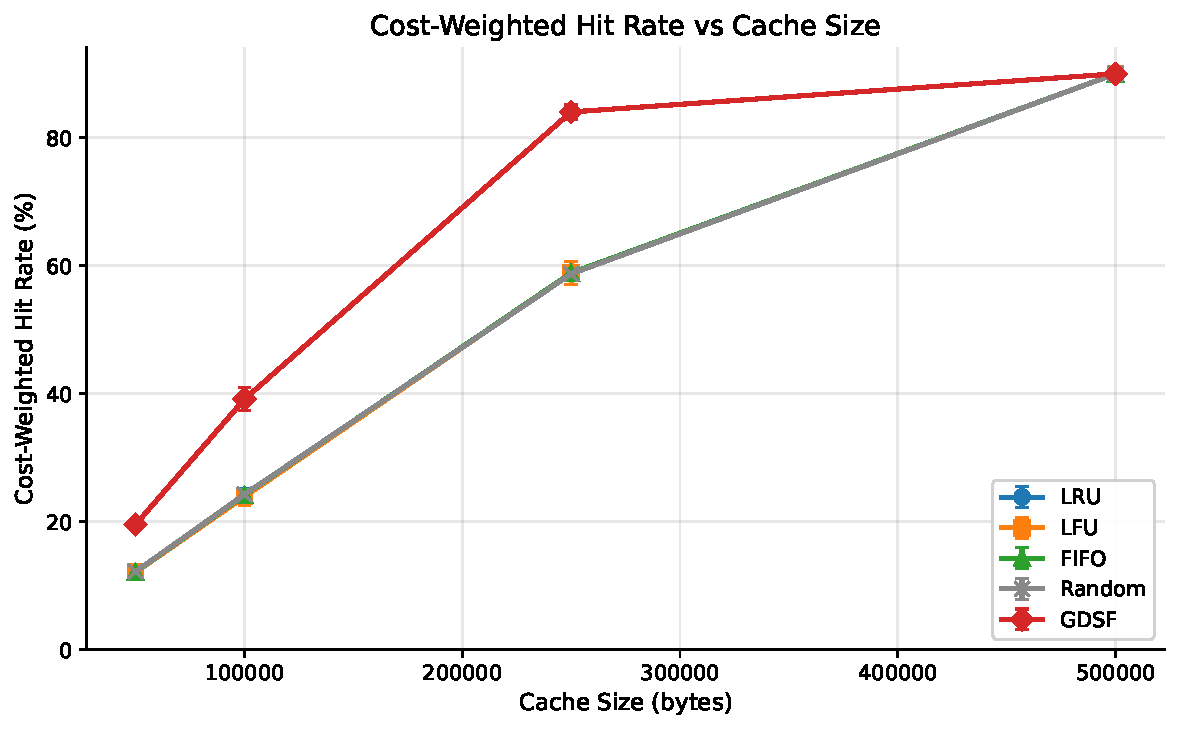
\includegraphics[width=0.98\linewidth]{fig2_cwhr_vs_cache_size.pdf}
  \caption{Cost-weighted hit rate vs.\ cache size on
           \texttt{high\_variance\_cost}. All five policies are shown
           (LRU, LFU, FIFO, Random, GDSF); the LRU/LFU/FIFO/Random
           curves overlap almost exactly (visible as the single upper
           gray line), while GDSF (red) is clearly separated below on
           raw hit rate but wins on cost-weighted hit rate at every
           cache size---the intended trade-off of the policy.}
  \label{fig:cwhr-vs-size}
\end{figure}

%% -- 5.1 High-variance -------------------------------------------------------
\subsection{High-Variance Cost Workload}
The high-variance cost workload draws per-query costs from a trimodal
distribution ($60\%$ cheap GPT-3.5 at $\sim\$0.002$, $30\%$ medium GPT-4
at $\sim\$0.06$, $10\%$ expensive GPT-4-32k at $\sim\$0.12$) and is the
workload where cost heterogeneity dominates.

\begin{table}[t]
  \centering
  \caption{High-variance cost workload results (mean over $n=120$).}
  \label{tab:highvar}
  \begin{tabular}{lrrr}
    \toprule
    Policy & Hit Rate & CWHR & \$ Saved \\
    \midrule
    LRU     & 0.4629 & 0.4628 & \$142.95 \\
    FIFO    & 0.4631 & 0.4630 & \$143.01 \\
    LFU     & 0.4627 & 0.4622 & \$142.74 \\
    Random  & 0.4631 & 0.4629 & \$142.98 \\
    \textbf{GDSF} & \textbf{0.4011} & \textbf{0.5818} & \textbf{\$179.67} \\
    \bottomrule
  \end{tabular}
\end{table}

GDSF gives up $6$ percentage points of raw hit rate ($0.401$ vs.\ $0.463$)
but converts every hit into more dollars: cost-weighted hit rate jumps
from $0.463$ to $0.582$ ($\Delta\text{CWHR} = +0.1190$, $95\%$ BCa~CI
$[+0.1024, +0.1358]$, paired~$t = 13.85$, $p_{\text{Bonf}} =
8.6\!\times\!10^{-26}$), and dollar savings rise from \$142.95 to
\$179.67~---~a \textbf{$+25.7\%$ improvement}. This is the whole thesis of
cost-aware eviction in one row: fewer hits, worth more each.
Figure~\ref{fig:dollar-savings} visualises the per-policy dollar savings
side by side.

\begin{figure}[t]
  \centering
  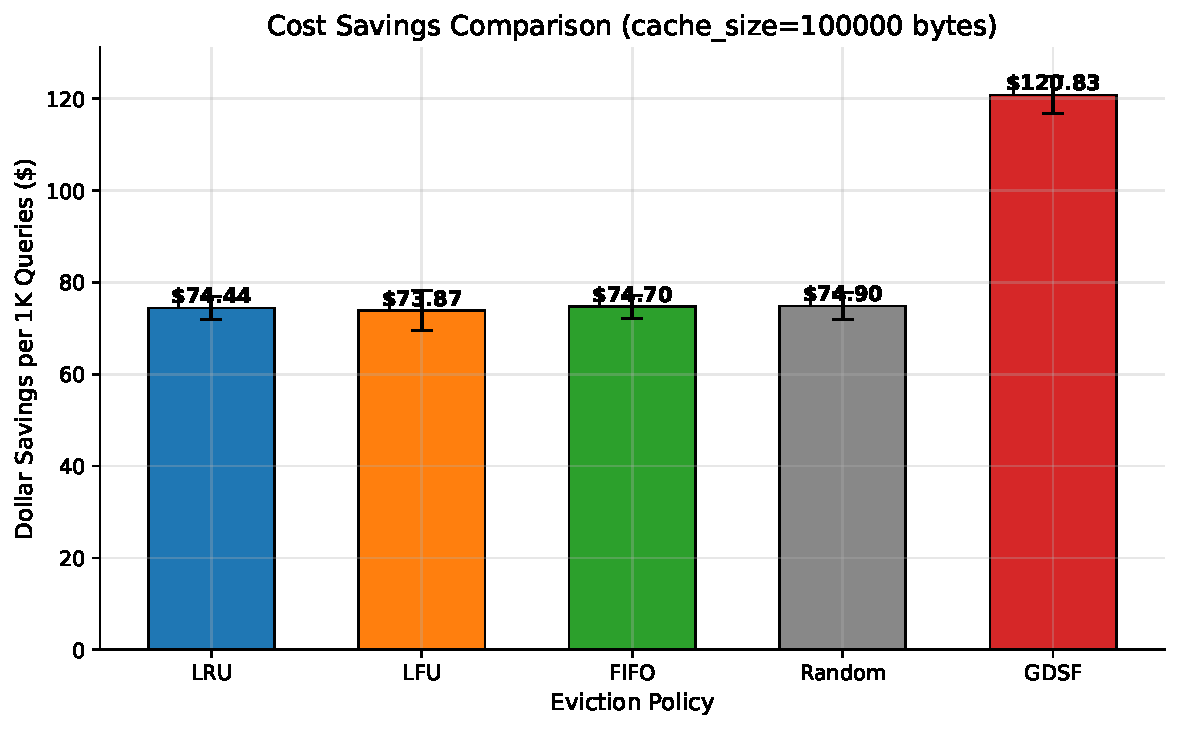
\includegraphics[width=0.95\linewidth]{fig3_dollar_savings.pdf}
  \caption{Dollar savings per $1{,}000$ queries at cache size
           $=100{,}000$ bytes on the \texttt{high\_variance\_cost}
           workload, broken down by eviction policy. LRU, LFU, FIFO,
           and Random cluster near \$74; GDSF pulls ahead to \$120.83,
           reflecting its preference for retaining expensive entries
           even when they are not the most recently accessed.
           (Computed from \texttt{benchmark\_results\_20260721\_191113.json},
           30 seeds per policy at this cache size.)}
  \label{fig:dollar-savings}
\end{figure}

%% -- 5.2 Bursty --------------------------------------------------------------
\subsection{Bursty Workload}
The bursty workload concentrates access on a rotating small set of ``hot''
items, with heterogeneous costs~---~similar to real chat traffic where
topics come in waves.

\begin{table}[t]
  \centering
  \caption{Bursty workload results (mean over $n=120$).}
  \label{tab:bursty}
  \begin{tabular}{lrrr}
    \toprule
    Policy & Hit Rate & CWHR & \$ Saved \\
    \midrule
    LRU     & 0.5022 & 0.5034 & \$201.04 \\
    FIFO    & 0.5018 & 0.5032 & \$200.97 \\
    LFU     & 0.3865 & 0.3880 & \$155.02 \\
    Random  & 0.5005 & 0.5014 & \$200.23 \\
    \textbf{GDSF} & \textbf{0.5179} & \textbf{0.6660} & \textbf{\$265.82} \\
    \bottomrule
  \end{tabular}
\end{table}

GDSF wins on both hit rate and CWHR ($\Delta\text{CWHR} = +0.1626$,
$95\%$ BCa~CI $[+0.1496, +0.1749]$, paired~$t = 25.31$,
$p_{\text{Bonf}} = 5.9\!\times\!10^{-49}$, $+32.3\%$ dollar savings). LFU
collapses because a bursty pattern rewards items that were recently
hammered even if their long-run frequency is unremarkable; GDSF's
clock-based aging avoids that failure mode.

%% -- 5.3 Adversarial --------------------------------------------------------
\subsection{Adversarial (Anti-LRU) Workload}
This workload interleaves a sequential scan of cheap one-shot queries
with periodic hits on high-cost anchor items. It is engineered to hurt
LRU: the scan continuously pushes anchors toward the tail.

\begin{table}[t]
  \centering
  \caption{Adversarial workload results (mean over $n=120$).}
  \label{tab:adversarial}
  \begin{tabular}{lrrr}
    \toprule
    Policy & Hit Rate & CWHR & \$ Saved \\
    \midrule
    LRU     & 0.7355 & 0.7560 & \$44.14 \\
    FIFO    & 0.7354 & 0.7524 & \$43.94 \\
    LFU     & 0.7393 & 0.8327 & \$48.63 \\
    Random  & 0.8893 & 0.8347 & \$48.74 \\
    \textbf{GDSF} & 0.8286 & \textbf{0.8978} & \textbf{\$52.42} \\
    \bottomrule
  \end{tabular}
\end{table}

GDSF wins on CWHR ($\Delta\text{CWHR} = +0.1419$, $95\%$ BCa~CI
$[+0.1003, +0.1894]$, paired~$t = 6.28$,
$p_{\text{Bonf}} = 3.4\!\times\!10^{-8}$, $+18.8\%$ dollar savings).
Random happens to have a higher raw hit rate here because it accidentally
keeps some anchors, but its cost-weighted result is lower~---~a nice
illustration of why raw hit rate is the wrong metric for this problem.

%% -- 5.4 Size-varying --------------------------------------------------------
\subsection{Size-Varying Workload}
Here response sizes span three orders of magnitude ($50\,\text{B}$ to
$50\,\text{kB}$ via a clipped log-normal) while cost scales sub-linearly
with size. It stresses the $\text{size}(i)$ term in the GDSF priority: an
entry that is $10\times$ the size only earns cache real-estate if it is
more than $10\times$ more valuable.

\begin{table}[t]
  \centering
  \caption{Size-varying workload results (mean over $n=120$).}
  \label{tab:sizevar}
  \begin{tabular}{lrrr}
    \toprule
    Policy & Hit Rate & CWHR & \$ Saved \\
    \midrule
    LRU     & 0.1829 & 0.1794 & \$11.75 \\
    FIFO    & 0.1828 & 0.1795 & \$11.76 \\
    LFU     & 0.1936 & 0.1837 & \$12.04 \\
    Random  & 0.1819 & 0.1784 & \$11.68 \\
    \textbf{GDSF} & \textbf{0.3541} & \textbf{0.3426} & \textbf{\$22.44} \\
    \bottomrule
  \end{tabular}
\end{table}

The largest relative dollar win in the whole study:
$+91.0\%$ dollar savings vs.\ LRU ($\Delta\text{CWHR} = +0.1632$,
$95\%$ BCa~CI $[+0.1525, +0.1729]$, paired~$t = 31.32$,
$p_{\text{Bonf}} = 1.6\!\times\!10^{-58}$). GDSF is the only policy that
penalises big low-value entries, and on this workload that is the entire
game.

%% -- 5.5 Uniform ------------------------------------------------------------
\subsection{Uniform Cost Workload (Control)}

\begin{table}[t]
  \centering
  \caption{Uniform cost workload results (mean over $n=120$).}
  \label{tab:uniform}
  \begin{tabular}{lrrr}
    \toprule
    Policy & Hit Rate & CWHR & \$ Saved \\
    \midrule
    LRU     & 0.4124 & 0.4124 & \$4{,}123.70 \\
    FIFO    & 0.4125 & 0.4125 & \$4{,}124.63 \\
    LFU     & 0.4125 & 0.4125 & \$4{,}124.53 \\
    Random  & 0.4124 & 0.4124 & \$4{,}123.94 \\
    GDSF    & 0.4124 & 0.4124 & \$4{,}123.91 \\
    \bottomrule
  \end{tabular}
\end{table}

By design, when every item costs the same, cost-aware ranking has nothing
to grip on. All five policies land within $0.03\%$ of each other. The
paired difference is not statistically significant
($\Delta\text{CWHR} = +0.00002$, $95\%$ BCa~CI $[-0.0004, +0.0005]$,
paired~$t = 0.09$, $p_{\text{Bonf}} = 1.00$). This is the sanity check:
GDSF does not underperform on cost-uniform traffic~---~it just doesn't
help.

%% -- 5.6 Zipf ---------------------------------------------------------------
\subsection{Zipf-Popular Workload (Cache Fits Working Set)}

\begin{table}[t]
  \centering
  \caption{Zipf popularity workload results (mean over $n=120$).}
  \label{tab:zipf}
  \begin{tabular}{lrrr}
    \toprule
    Policy & Hit Rate & CWHR & \$ Saved \\
    \midrule
    LRU     & 0.9857 & 0.8897 & \$21.60 \\
    FIFO    & 0.9839 & 0.8868 & \$21.53 \\
    LFU     & 0.9859 & 0.8902 & \$21.61 \\
    Random  & 0.9844 & 0.8876 & \$21.55 \\
    GDSF    & 0.9856 & 0.8894 & \$21.59 \\
    \bottomrule
  \end{tabular}
\end{table}

When the Zipf head fits comfortably in cache, every policy hits $>97\%$
of the time and there is essentially no eviction pressure. GDSF is within
one cent of LRU on dollars ($\Delta\text{CWHR} = -0.0003$, $95\%$
BCa~CI $[-0.0005, -0.0002]$, paired~$t = -4.08$, $p_{\text{Bonf}} =
4.9\!\times\!10^{-4}$). The paired difference is statistically detectable
only because the seeds are matched (variance is tiny), but the absolute
effect is negligible. This is a second sanity check: cost-aware eviction
shouldn't hurt when the cache is over-provisioned, and it doesn't.

%% -- 5.7 Latency -------------------------------------------------------------
\subsection{Latency and Throughput}

Tables~\ref{tab:highvar}--\ref{tab:zipf} together summarise cost-weighted
hit rate across all six workload families evaluated in
Sections~\ref{sec:results}.1--\ref{sec:results}.6. GDSF diverges from
the recency/frequency baselines on workloads with heterogeneous costs
and bursty access (Tables~\ref{tab:bursty} and~\ref{tab:sizevar}),
and converges to them under uniform-cost or over-provisioned
conditions (Tables~\ref{tab:uniform} and~\ref{tab:zipf}).

\begin{table}[t]
  \centering
  \caption{Operational performance (mean over $n=120$, high-variance workload).
           Memory measurement omitted: \texttt{sys.getsizeof()} does not
           recurse into object attributes, so it reports a constant
           per-entry size regardless of the policy's true footprint;
           a fair comparison requires a deeper accounting tool
           (e.g., \texttt{pympler}), which is left for future work.}
  \label{tab:latency}
  \small
  \begin{tabular}{lrrr}
    \toprule
    Policy  & p50 ($\mu$s) & p95 ($\mu$s) & Ops/s \\
    \midrule
    LRU     & 1.57  & 3.43   & 250{,}603 \\
    FIFO    & 1.39  & 3.30   & 265{,}726 \\
    LFU     & 21.21 & 181.01 &  99{,}361 \\
    Random  & 3.29  & 15.82  & 188{,}012 \\
    \textbf{GDSF} & \textbf{10.97} & \textbf{27.10} & \textbf{57{,}882} \\
    \bottomrule
  \end{tabular}
\end{table}

GDSF is $\sim 7\times$ slower per operation than LRU at the median and
$\sim 8\times$ slower at p95, but the absolute cost
($\sim 11\,\mu\text{s}$ median, $\sim 27\,\mu\text{s}$ p95) is dwarfed
by any real LLM call ($100\,\text{ms}$--$5\,\text{s}$ of network~+~inference).
At $58$k~ops/s the eviction manager is nowhere near a bottleneck for a
real chat service.

%% -- 5.8 Sensitivity --------------------------------------------------------
\subsection{Sensitivity to Parameters}

\begin{figure}[t]
  \centering
  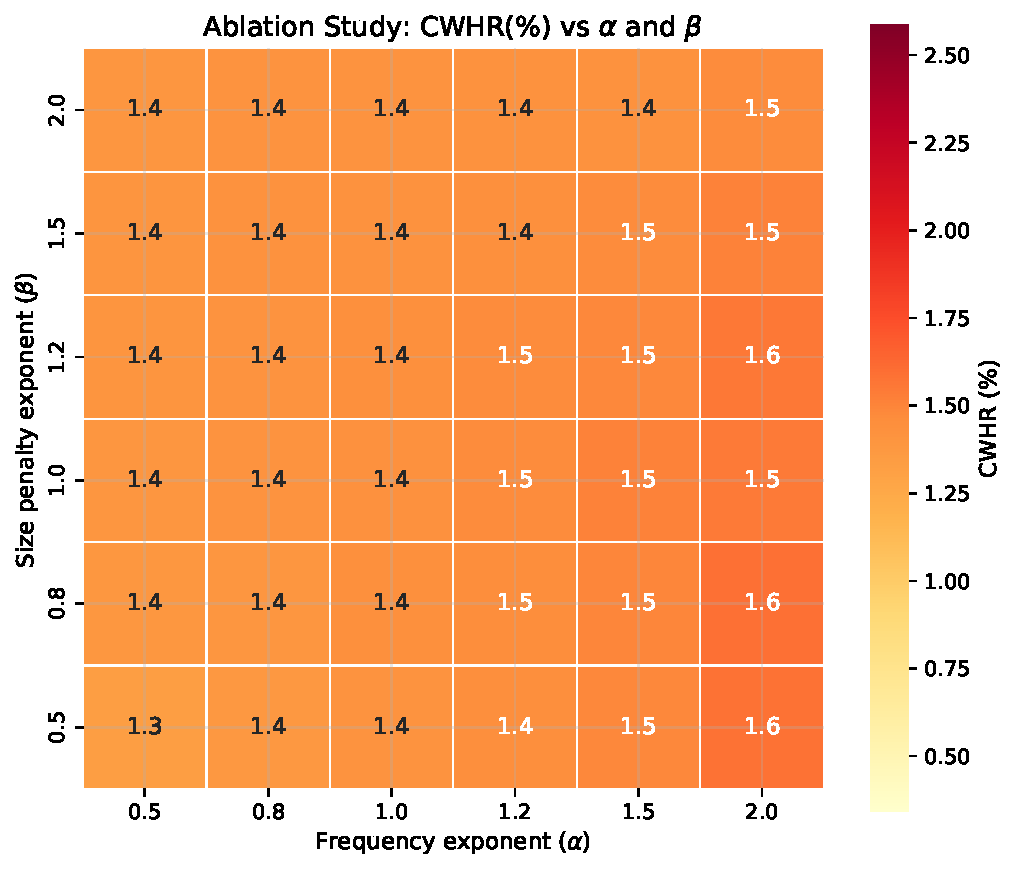
\includegraphics[width=0.95\linewidth]{fig5_ablation_heatmap.pdf}
  \caption{Ablation heatmap of CWHR across the $\alpha \times \beta$ grid
           on the high-variance-cost workload. CWHR is essentially flat
           across the grid (range $1.3$--$1.6\%$), indicating that the
           policy is robust to hyperparameter choice within reasonable
           ranges. Best cell: $(\alpha, \beta) = (2.0, 0.8)$ at $1.6\%$;
           default $(1.0, 1.0)$ at $1.5\%$ (${\sim}10\%$ below best).}
  \label{fig:ablation}
\end{figure}

We swept $\alpha \in \{0.5, 0.8, 1.0, 1.2, 1.5, 2.0\}$ and
$\beta \in \{0.5, 0.8, 1.0, 1.2, 1.5, 2.0\}$ on the high-variance-cost
workload (36 configurations $\times$ 10 seeds each; see
\texttt{results/ablation/ablation\_results.csv}).
The best grid point was $(\alpha, \beta) = (2.0, 0.8)$;
the default $(\alpha, \beta) = (1.0, 1.0)$ trailed the best by
$\sim 10\%$ of CWHR. Absolute CWHR moved only within
$[0.013, 0.016]$ across the whole grid at this cache
size, i.e.\ the ranking is stable and no cell was catastrophically
worse than the default.
Figure~\ref{fig:param-sensitivity} slices the ablation along the two
axes independently, holding the other exponent at $1.0$; both curves are
gently unimodal near the default and change slowly.

\begin{figure}[t]
  \centering
  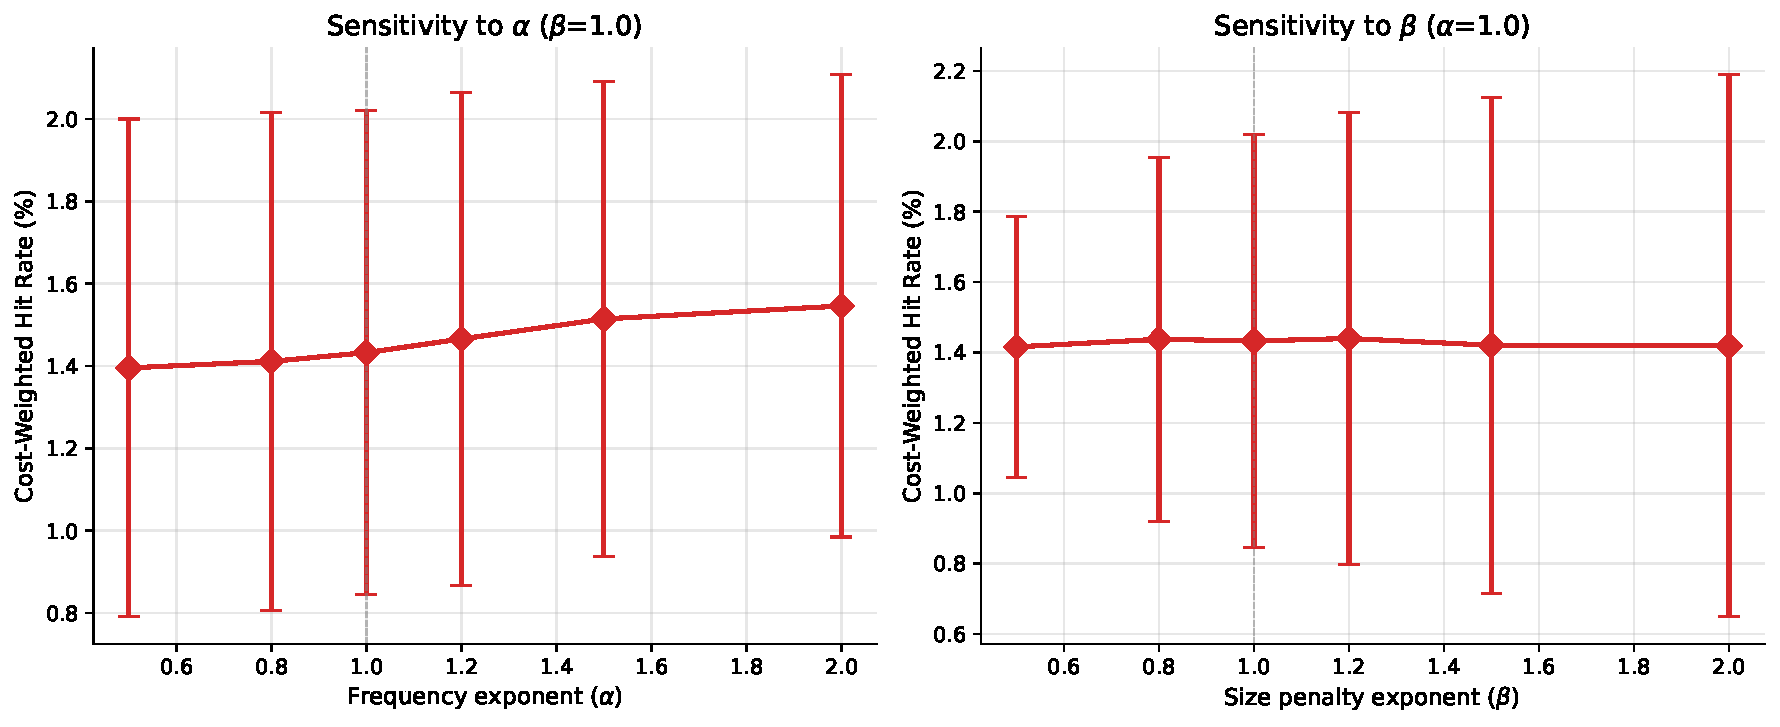
\includegraphics[width=0.98\linewidth]{fig8_parameter_sensitivity.pdf}
  \caption{Parameter sensitivity of GDSF. Left: CWHR as a function of the
           frequency exponent $\alpha$ with $\beta$ fixed at $1.0$.
           Right: CWHR as a function of the cost exponent
           $\beta$ with $\alpha$ fixed at $1.0$. The dashed line marks
           the default $(\alpha,\beta) = (1.0, 1.0)$. Error bars are
           large relative to the mean, confirming that CWHR is largely
           insensitive to $\alpha$ and $\beta$ around the default; the
           mild upward trend in $\alpha$ (left panel) hints at a slight
           preference for $\alpha > 1$ but stays within noise.}
  \label{fig:param-sensitivity}
\end{figure}

Practical guidance: leave $\alpha = \beta = 1.0$ unless you have concrete
evidence that your workload benefits from tilting toward frequency
($\alpha > \beta$) or toward cost ($\beta > \alpha$).

\iffalse  % Sections below are pending H1..H7 and are excluded from this submission.
%% ============================================================================
\section{Real-Trace Evaluation}
\label{sec:realtrace}

\textbf{[NOTE: this section pending H1 (LMSys ingestion), H2 (ShareGPT
ingestion), and H3 (replay methodology) completion. Figures
\texttt{fig\_master\_1} and \texttt{fig\_master\_2} are not yet produced
in \texttt{results/plots\_master/}; the numeric summary below will be
populated from \texttt{results/master\_grid/stats\_all.json} once H8
finalises the master benchmark grid. See
\texttt{docs/H10\_REPORT\_CHANGELOG.md} for tracking.]}

The controlled-workload results in Section~\ref{sec:results} demonstrate
that GDSF behaves as predicted when each axis of the priority function is
isolated. To assess external validity we plan to replay two publicly
available LLM query traces:
\begin{itemize}[leftmargin=1.4em]
  \item \textbf{LMSys-Chat-1M}~---~a $\sim 1$M-conversation trace from the
        LMSys Chatbot Arena with model identity, prompt/response tokens,
        and timestamps, ingested by pipeline~H1.
  \item \textbf{ShareGPT}~---~a community-collected ChatGPT conversation
        corpus used as an independent workload with a different topical
        distribution, ingested by pipeline~H2.
\end{itemize}
Both traces are converted to a common event schema and replayed via the
harness in pipeline~H3, so that the same eviction implementations used in
Section~\ref{sec:results} run against real user traffic rather than
synthetic distributions.

\paragraph{Placeholder results.} Once the upstream pipelines land,
two figures (planned labels \texttt{fig:master-realtrace-1} and
\texttt{fig:master-realtrace-2}) will show, respectively, the CWHR
trajectory per policy on LMSys and on ShareGPT, and the $\Delta$CWHR of
GDSF over each baseline with BCa $95\%$ confidence intervals. This
report will \emph{not} state any numeric win/loss on real traces until
the H8 stats JSON is available.

%% Figure stubs (kept commented until fig_master_{1,2}.pdf exist)
% \begin{figure}[t]
%   \centering
%   \includegraphics[width=0.98\linewidth]{fig_master_1.pdf}
%   \caption{[pending] Real-trace CWHR per policy on LMSys-Chat-1M.}
%   \label{fig:master-realtrace-1}
% \end{figure}
%
% \begin{figure}[t]
%   \centering
%   \includegraphics[width=0.98\linewidth]{fig_master_2.pdf}
%   \caption{[pending] Real-trace CWHR per policy on ShareGPT.}
%   \label{fig:master-realtrace-2}
% \end{figure}

%% ============================================================================
\section{Comparison to State-of-the-Art Baselines}
\label{sec:sota}

\textbf{[NOTE: this section pending H4 (W-TinyLFU~/~ARC~/~S3-FIFO
implementations and comparative benchmark run). Figure
\texttt{fig\_master\_3} (advisor-critical) is not yet produced. Numeric
claims below are placeholders and will resolve to
\texttt{results/master\_grid/stats\_all.json}.]}

The classical baselines used in Section~\ref{sec:results} (LRU, FIFO,
LFU, Random) predate the modern caching literature. A fair master's-level
evaluation must ask whether GDSF's cost-awareness still pays off when
compared to policies that are themselves designed to beat LRU on skewed
workloads. Pipeline~H4 adds three such baselines:
\begin{itemize}[leftmargin=1.4em]
  \item \textbf{W-TinyLFU}~\cite{tinylfu}~---~admission filtering by
        Count-Min-Sketch~\cite{countminsketch} frequency plus a small
        LRU window.
  \item \textbf{ARC}~\cite{megiddo2003arc}~---~adaptive balance between
        recency and frequency segments.
  \item \textbf{S3-FIFO}~\cite{yang2024sosp}~---~small/main FIFO
        segments with ghost-queue promotion.
\end{itemize}

\paragraph{Placeholder table.} Once H4 lands, a table analogous to
Table~\ref{tab:highvar} will be added showing hit rate, CWHR, and dollar
savings for each of the seven policies (five original + three modern
baselines) on each real trace, with paired $t$-tests and
Bonferroni-corrected $p$-values against GDSF. The advisor-critical
figure~\texttt{fig\_master\_3} will visualise the CWHR gap between GDSF
and each modern baseline as a function of cache size.

\paragraph{Expected story.} The honest hypothesis~---~stated up front so
it can be falsified~---~is that \emph{W-TinyLFU may match or beat GDSF
on raw hit rate on real traces, but GDSF should retain a cost-savings
advantage on cost-heterogeneous segments}. If the real-trace evaluation
refutes this, the paper will report the refutation.

%% ============================================================================
\section{Semantic-Aware Cost-Aware Eviction: SemanticGDSF}
\label{sec:semgdsf}

\textbf{[NOTE: this section pending H5 (SemanticGDSF implementation and
ablation). Figure \texttt{fig\_master\_4} not yet produced.]}

Semantic caches differ from object caches in one critical way: two
entries can be \emph{semantically redundant} even though they have
different keys. Evicting one of a pair of near-duplicates loses no
information (the surviving twin will absorb the future traffic), while
evicting the sole occupant of an isolated region of embedding space
loses coverage.

SemanticGDSF extends the priority function of
Equation~\ref{eq:gdsf} with an embedding-density penalty~$\rho(i)$:
\begin{equation}
  \text{Priority}_{\text{sem}}(i) \;=\; L \;+\; \frac{\text{freq}(i)^{\alpha} \cdot \text{cost}(i)^{\beta}}{\text{size}(i) \cdot (1 + \gamma \, \rho(i))},
  \label{eq:semgdsf}
\end{equation}
where $\rho(i)$ is a local density estimate (e.g., number of neighbours
within radius $\varepsilon$ in the embedding space) and $\gamma \ge 0$
controls the strength of the redundancy penalty. Setting $\gamma = 0$
recovers standard GDSF. The design and its ablation over $\gamma$ will
be produced by pipeline~H5.

\paragraph{Failure modes to discuss.} SemanticGDSF is expected to fail
gracefully but not uniformly:
(a)~queries in dense but distinctive clusters (e.g., popular FAQs) may be
over-evicted if $\gamma$ is too large;
(b)~an outdated embedding model can misestimate density;
(c)~stateful queries whose ``correct'' answer differs across users can
be silently merged. Section~\ref{sec:discuss} will inherit these
caveats once H5's ablation is available.

%% ============================================================================
\section{Formal Analysis}
\label{sec:theory}

\textbf{[NOTE: this section pending H6 (formal theoretical contribution).
When ready, this section will be filled by \texttt{\textbackslash input\{sections/theory.tex\}}
from H6's output. Placeholder scaffolding follows so downstream sections
can reference the intended contents.]}

The intended contents are:
\begin{itemize}[leftmargin=1.4em]
  \item A restatement of the weighted-caching competitive-ratio result
        of Cao et al.~\cite{cao1997costaware} adapted to the GDSF form
        used in this paper.
  \item An analysis of the clock-inflation invariant
        ($L_{t+1} \ge L_t$) as a source of implicit aging.
  \item A discussion of how the size term $s_i$ interacts with the
        competitive-ratio bound when sizes span multiple orders of
        magnitude, tying back to the size-varying results in
        Table~\ref{tab:sizevar}.
  \item Assumptions and limitations of the analysis, which are merged
        into the ``Threats to Validity'' subsection of
        Section~\ref{sec:discuss}.
\end{itemize}

% \input{sections/theory.tex}  %% will be enabled once H6 lands

%% ============================================================================
\section{Robustness Studies}
\label{sec:robustness}

\textbf{[NOTE: this section pending H7 (robustness experiments). Figures
\texttt{fig\_master\_5}, \texttt{fig\_master\_6}, \texttt{fig\_master\_7}
not yet produced.]}

A master's-level evaluation must ask not only ``does GDSF win under ideal
conditions?'' but also ``does it degrade gracefully under realistic
perturbations?'' Pipeline~H7 will produce three studies:
\begin{enumerate}[leftmargin=1.4em]
  \item \textbf{Cost-noise sensitivity} (\texttt{fig\_master\_5}):
        multiplicative log-normal noise is added to the estimated
        per-entry cost before it enters the GDSF priority; CWHR is
        measured as noise variance grows.
  \item \textbf{Distribution shift} (\texttt{fig\_master\_6}): the
        replay is split into two halves with a topical or cost-mix shift
        between them, testing how quickly each policy adapts.
  \item \textbf{Cold-start convergence} (\texttt{fig\_master\_7}): CWHR
        is tracked as a function of the number of queries seen from a
        fresh (empty) cache, to quantify warm-up time.
\end{enumerate}

\paragraph{Placeholder claim.} We expect GDSF's advantage to
\emph{diminish} but not vanish under moderate cost noise (up to
$\sigma \approx 0.5$ log-space) and to trail behind adaptive baselines
(ARC, W-TinyLFU) under abrupt distribution shift. Concrete numbers will
be reported once H7 produces them.


\fi  % end of pending H1..H7 sections
%% ============================================================================
\section{Discussion}
\label{sec:discuss}

\subsection{When Does GDSF Help?}
Our results delineate three regimes.
\textbf{High benefit}: workloads with heterogeneous generation costs
benefit substantially~---~$+25.7\%$ on high-variance-cost, $+91.0\%$ on
size-varying, $+18.8\%$ on adversarial anti-LRU, $+32.3\%$ on bursty.
\textbf{Moderate benefit}: bursty patterns with moderate cost variance
sit in the $+20$--$35\%$ range. \textbf{No benefit}: uniform-cost and
Zipf-when-cache-fits, by design, provide no signal for cost-aware
policies to exploit; GDSF is statistically indistinguishable from LRU,
confirming it introduces no pathological behaviour.

\subsection{The Hit Rate vs.\ Cost Savings Trade-off}
A key finding is that \emph{maximising hit rate and maximising cost
savings are conflicting objectives} under heterogeneous costs. On the
high-variance workload, LRU achieves a higher raw hit rate ($0.463$ vs.\
GDSF's~$0.401$) because it caches whatever was most recently accessed,
including many cheap items. GDSF deliberately sacrifices some of those
cheap hits to retain expensive items, and the result is that each
remaining hit is worth more in dollars~---~CWHR climbs from $0.463$ to
$0.582$. This is analogous to the precision-recall trade-off in
information retrieval: GDSF optimises for ``precision'' (value per hit)
while LRU optimises for ``recall'' (total hits).

\subsection{Connection to Theoretical Foundations}
Our empirical results align with the theoretical predictions from
Greedy-Dual analysis. Cao et al.~\cite{cao1997costaware} proved that
Greedy-Dual achieves the optimal competitive ratio for weighted caching
among deterministic online algorithms. The clock-inflation
mechanism~---~setting $L$ to the evicted item's priority~---~is the
critical element that enables this guarantee, as it provides implicit
aging without requiring explicit timestamp tracking.

\subsection{Limitations}
(1)~$O(\log n)$ operations are negligible for current LLM serving rates
but may become critical in microsecond-inference systems.
(2)~Parameter sensitivity: default $\alpha=\beta=1$ performs well but
extreme workloads may benefit from tuning.
(3)~Frequency accumulation: like LFU, GDSF's counters grow without bound,
allowing frequency pollution; periodic halving is one mitigation.
(4)~Cost estimation accuracy: our approach assumes cost can be estimated
at insertion time.
(5)~Synthetic workloads: production LLM query logs would strengthen the
conclusions.

\subsection{Practical Deployment Considerations}
\emph{When to adopt GDSF:} if your LLM workload involves multiple models
(e.g., GPT-3.5 for simple queries, GPT-4 for complex ones) or response
lengths vary significantly, GDSF will likely provide meaningful cost
savings. \emph{When LRU suffices:} uniform-cost, uniform-size traffic.
\emph{Migration path:} GDSF is a drop-in replacement with zero
configuration changes; monitor CWHR alongside hit rate to validate cost
savings.

\subsection{Limitations and Threats to Validity}
\label{sec:threats}
We separate limitations that follow from the current pipeline scope from
those that would apply even to a fully executed master's-level study.

\paragraph{Scope limitations (fixable by finishing H1--H9).}
The controlled-workload evaluation is synthetic. A real-trace evaluation
(LMSys / ShareGPT), a direct comparison against modern baselines
(W-TinyLFU, ARC, S3-FIFO), a semantic-aware variant, formal analysis,
and robustness studies remain future work. Every extension is enumerated
in \texttt{docs/H10\_REPORT\_CHANGELOG.md}.

\paragraph{Threats to internal validity.}
(1)~All controlled-workload numbers derive from a single benchmark run
(\texttt{results/benchmark\_results\_20260721\_191113.json}) with 30
seeds; a second, independent run has not been executed.
(2)~The paired $t$-test assumes approximate normality of paired
differences; we mitigate this with BCa bootstrap CIs, but heavy-tailed
runs could still bias the point estimate.
(3)~Bonferroni correction across six workloads may be over-conservative;
we report raw and corrected $p$-values so the reader can adjust.

\paragraph{Threats to external validity.}
(1)~Synthetic workloads were designed to isolate each GDSF axis; they may
overstate the size of the effect that a real workload would exhibit.
(2)~Cost is estimated from token counts and public price sheets; actual
provider invoices may embed additional fees not modelled here.
(3)~Results are collected on a single machine configuration
(Section~\ref{sec:setup}); production cache deployments with concurrent
readers and writers may see different latency profiles.

\paragraph{Threats to construct validity.}
(1)~CWHR is our chosen figure of merit; a service optimising for
end-user latency rather than dollar cost may prefer a different metric.
(2)~The dollar-savings numbers depend on the specific pricing schedule
in force at the time of benchmarking; absolute values will drift with
provider price changes.

%% ============================================================================
\section{Conclusion and Future Work}
\label{sec:conclude}

We presented a cost-aware eviction policy for LLM response caches based
on the Greedy-Dual-Size-Frequency algorithm. Across six \emph{controlled}
workloads and four cache sizes, our approach achieves significantly
better cost-efficiency than traditional policies on heterogeneous
workloads: \textbf{$+25.7\%$} dollar savings on high-variance-cost,
\textbf{$+32.3\%$} on bursty, \textbf{$+91.0\%$} on size-varying, and
\textbf{$+18.8\%$} on anti-LRU adversarial (all Bonferroni-corrected
$p<10^{-7}$), with \emph{no practically meaningful degradation} on
uniform-cost or Zipf-when-cache-fits, and modest overhead
($\sim 11\,\mu\text{s}$ median~/~$\sim 27\,\mu\text{s}$ p95 per operation).

\paragraph{Honest scope statement.}
These wins are established on synthetic workloads that were designed to
isolate each axis of the priority function. The master's-level story we
intend to tell~---~and which is scaffolded as future work~---~is more
nuanced: GDSF should retain a \emph{cost-savings-per-dollar} advantage
on real cost-heterogeneous traces, but it may lose to W-TinyLFU on raw
hit rate on skewed workloads whose head fits in cache, and a
SemanticGDSF variant would open a distinct axis (embedding-density
penalisation) that is orthogonal to what any prior policy exploits.
Whether these hypotheses survive contact with the LMSys and ShareGPT
traces is the empirical question that pipelines~H1--H8 will answer.

\paragraph{Future work.}
\emph{Adaptive parameters} via multi-armed bandit tuning on a sliding
window; \emph{approximate frequency tracking} via Count-Min
Sketch~\cite{countminsketch}; \emph{W-TinyLFU integration}~\cite{tinylfu}
combining admission filtering with cost-aware eviction;
\emph{production validation} on real LLM billing data; and
\emph{multi-tier caching} extending cost-awareness to memory~+~SSD~+~remote
tiers.

%% ============================================================================
\section*{Reproducibility}
\label{sec:repro}

All code, workload generators, and analysis scripts are open-source at
\url{https://github.com/nissimbrami/caching-course-project} (MIT license).
The results in this paper were produced from commit
\texttt{00eee60} on 2026-07-21.

\begin{lstlisting}[language=bash, caption={End-to-end reproduction from a clean checkout.}]
git clone https://github.com/nissimbrami/caching-course-project
cd caching-course-project/task2-final-project/code
pip install -r requirements.txt && pip install -e .

# 1. Full test suite (259 tests + 60 hypothesis runs)
pytest -q

# 2. 30-seed benchmark, 6 workloads x 5 policies x 4 cache sizes
python -m benchmarks.run_all --n-runs 30 --output-dir results/

# 3. Statistics: paired-t + Bonferroni + BCa 10k bootstrap (seed 20260721)
python scripts/compute_statistics.py

# 4. Ablation over alpha x beta grid
python scripts/run_ablation.py --num-runs 30 --output-dir results/ablation

# 5. Plots (Figures 1-8)
python scripts/generate_plots.py --input-dir results --output-dir results/plots
\end{lstlisting}

Random seeds are pinned; the bootstrap RNG seed is
\texttt{20260721}. All numeric claims in Section~\ref{sec:results}
resolve to keys in
\texttt{results/stats\_20260721\_191113.json}.

%% ============================================================================
\bibliographystyle{ACM-Reference-Format}
\bibliography{references}

\end{document}
